\subsection{Benchmarking instances}

This section explains the two sets of benchmarks used.The medium size instance set consists of 38 small or medium size instances, and the large size instance set consists of 200 problem instances. The medium size set is used to compare the ILP model versus the Metaheuristics models. The large size set is used to test parameter values in order to find the best performing setup for each BRKGA and GRASP model, and finally to compare them solving one large problem instance.


\subsubsection{The instance generation process}

The algorithm used to generate problem instances is based on generating random but valid schedules of nurses and then adding the number of nurses working at each hour to compute the demand. This approach assures that the problem instance will always have a solution. Besides that, the algorithm places the schedules close to few selected hours of the schedule (adding some variability). The input values of the algorithm are all the variables of the problem instance, the selected hours of the schedule to place nurse schedules around and some proportion of extra nurses to add to the problem without using them to create the demand.


\subsubsection{The medium and large instance sets}


To decide how the size of a problem is determined, we choose to reference the time it takes for the ILP model to solve the problem instance using the Cplex solver. We generate and solve a series of instances with the ILP until we have around 20 instances that take 60 minutes or less to solve by ILP. Then, as we cannot perform the same procedure to generate the large instance set, we execute a series of experiments to determine the influence of the problem variables to the steps the ILP model has to do to decrease the gap between the best integer and the best bound.

The results are shown in figure~\ref{fig_ilp_size}, figure~\ref{fig_ilp_size2} and figure~\ref{fig_ilp_size3} page~\pageref{fig_ilp_size}. The table~\ref{tab:ilp_size} page~\pageref{tab:ilp_size} summarizes the findings and shows how we applied them to create the large benchmark instance set.

\begin{figure}[h!]

\begin{subfigure}[b]{.49\linewidth}
\centering
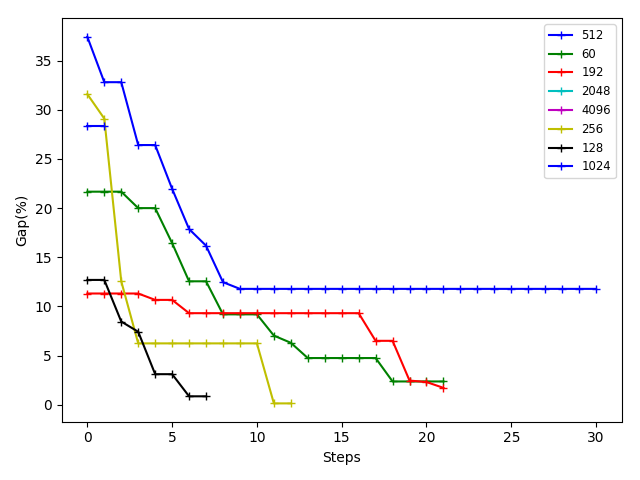
\includegraphics[width=\linewidth]{./img/instances_nurses_ilp_evol.png}
\caption{ Evolution of Gap of the ILP model with different number of nurses}\label{fig1a}
\end{subfigure}%
\begin{subfigure}[b]{.49\linewidth}
\centering
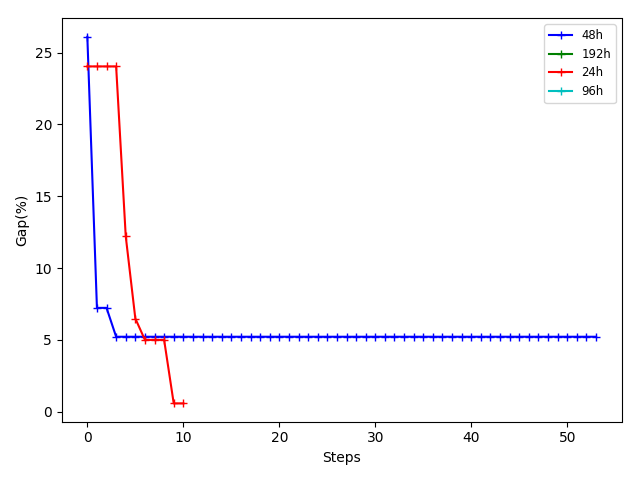
\includegraphics[width=\linewidth]{./img/instances_hours_ilp_evol.png}
\caption{ Evolution of Gap of the ILP model with different number of hours }\label{fig1b}
\end{subfigure}\vfill
\caption{Evolution of Gap of the ILP model with different values of number of nurses (\subref{fig1a}) and number of hours (\subref{fig1b}). }
\label{fig_ilp_size}
\end{figure}


\begin{figure}[h!]
\begin{subfigure}[b]{.49\linewidth}
\centering
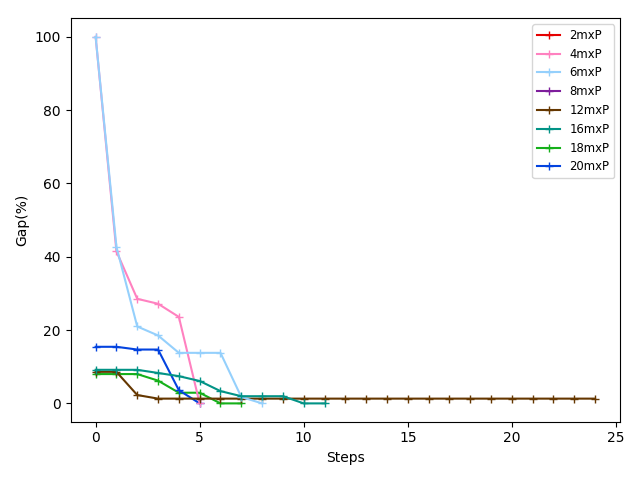
\includegraphics[width=\linewidth]{./img/instances_maxpresence_ilp_evol.png}
\caption{Evolution of Gap of the ILP model with different values of maxPresence parameter }\label{fig1c}
\end{subfigure}
\begin{subfigure}[b]{.49\linewidth}
\centering
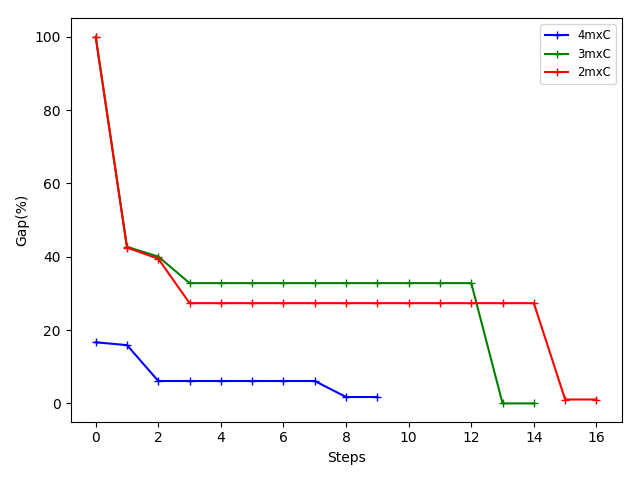
\includegraphics[width=\linewidth]{./img/instances_maxconsec_ilp_evol.png}
\caption{Evolution of Gap of the ILP model with different values of maxConsec parameter }\label{fig1d}
\end{subfigure}
\caption{Evolution of Gap of the ILP model with different values of maxPresence (\subref{fig1c}) and maxConsec (\subref{fig1d}).  }
\label{fig_ilp_size2}
\end{figure}


\begin{figure}[h!]
\begin{subfigure}[b]{.49\linewidth}
\centering
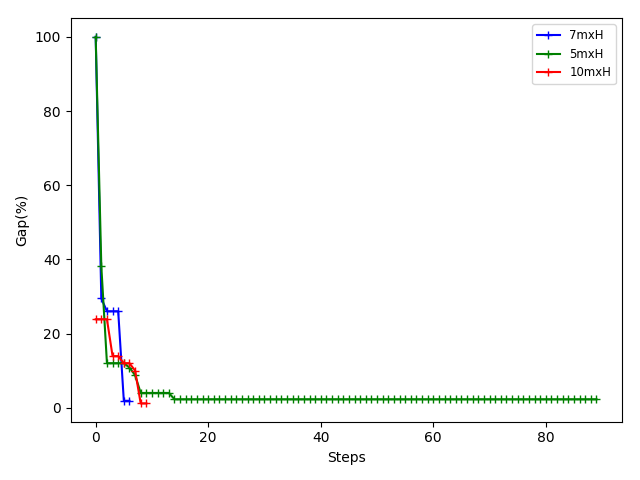
\includegraphics[width=\linewidth]{./img/instances_maxhours_ilp_evol.png}
\caption{Evolution of Gap of the ILP model with different values of maxHours parameter }\label{fig1c}
\end{subfigure}
\begin{subfigure}[b]{.49\linewidth}
\centering
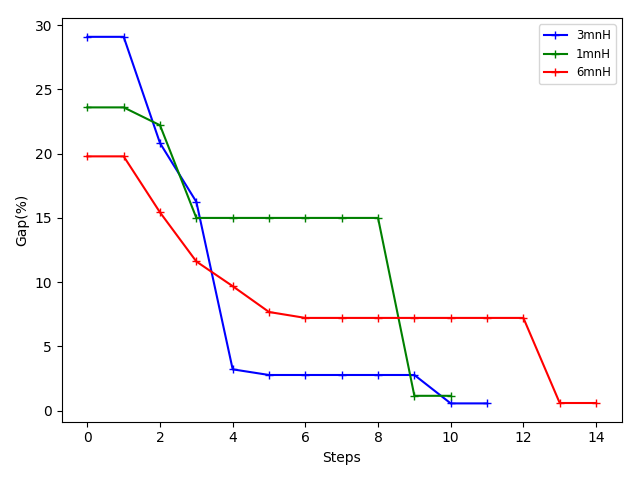
\includegraphics[width=\linewidth]{./img/instances_minhours_ilp_evol.png}
\caption{Evolution of Gap of the ILP model with different values of minHours parameter }\label{fig1d}
\end{subfigure}
\caption{Evolution of Gap of the ILP model with different values of maxHours (\subref{fig1c}) and minHours (\subref{fig1d}).  }
\label{fig_ilp_size3}
\end{figure}




\begin{table}[ht] 
\centering 
\begin{tabularx}{0.75\textwidth}{|l|c|c|c|}
\hline
\textbf{Problem} & \textbf{Effect on problem size}  & \textbf{Medium size set} & \textbf{Large size set} \\

\textbf{Variable}  		& \textbf{when increasing}  & 38 instances &  199 instances \\
\hline
\textbf{$nNurses$} & increases      &  64	&  64 to 4096 \\
\textbf{$hour$}   & increases		& 24	&  24, 48, 72 \\
\textbf{$maxPrensce$} & decreases	& 16	& 8 to 27 \\
\textbf{$maxConsec$} & decreases		& 5	&  4 to 13		\\
\textbf{$maxHours$} & decreases		& 4 to 10	& 2 to 12 \\
\textbf{$minHours$} & increases		& 1 to 5	& 1 to 9\\
\hline
\end{tabularx}
\caption{Benchmark datasets and variables influence on problem size}
\label{tab:ilp_size}
\end{table}


